\documentclass[a4paper,14pt]{extarticle}
% Стандартные формульные пакеты
\usepackage{float,amsmath,esint,amsfonts,wrapfig,bbm}
\usepackage{indentfirst}
\usepackage[usenames]{color}
\usepackage{multirow}
%выставляем поля
\usepackage[left=2cm,right=2cm,top=2cm,bottom=2cm,bindingoffset=0cm]{geometry}
% Русский текст в формулах
\usepackage{mathtext}
% Подключение русского языка
\usepackage[T2A]{fontenc}
\usepackage[english,russian]{babel}
\usepackage[utf8]{inputenc}
% Рисунки
\usepackage{graphicx,caption,subcaption}
% Landscape page
\usepackage{lscape}
\renewcommand{\arraystretch}{1.1}

\newcommand{\mymean}[3]{\left\langle #1 \left| #2 \right| #3 \right\rangle}
\newcommand{\myint}[2]{\langle #1 | #2 \rangle}
\newcommand{\myexp}[1]{\text{exp}\left( #1 \right)}
\newcommand{\myl}[0]{\mathit{L}}
\begin{document}
\section{Гармонический осциллятор}
Рассмотрим динамику Гауссовых волновых пакетов в гармоническом потенциале:
$$|\Psi\rangle = \sum_k D_k|g_k\rangle$$
$$V = \frac{1}{2}m\omega^2x^2,\ \dot{q}_k=\frac{p_k}{m},\ \dot{p}_k=-\left.\frac{\partial V}{\partial x}\right|_{q_k}=-m\omega^2q_k $$
$$\dot{\vec{D}} = -\frac{i}{\hbar}\mathbbm{S}(\mathbbm{H}-i\hbar\tau)\vec{D}$$
Для удобства проведем замену переменных:
$$g_k=N\myexp{\frac{1}{\hbar}\left(-\frac{1}{2}m\omega(x-q_k)^2+ip_kx\right)}=%
       \myexp{\frac{1}{\hbar}\left(-\frac{1}{2}m\omega x^2 + \xi_kx + \eta_k\right)}$$
$$\xi_k=m\omega q_k+ip_k,\ \eta_k=\hbar\ln N-\frac{1}{2}m\omega q_k^2$$
$$\dot{\xi}_k=m\omega\dot{q}_k+i\dot{p}_k=\omega p_k-im\omega^2q_k=-\omega(im\omega q_k - p_k)=-i\omega(m\omega q_k+ip_k)=-i\omega\xi_k$$
$$\dot{\eta}_k=-m\omega q_k\dot{q}_k=-\omega q_kp_k$$

Получим явный вид некоторых матричных элементов:
\begin{enumerate}
\item элементы матрицы перекрывания:
$$\mathbbm{S}_{mk}=\myint{g_m}{g_k}=\int\myexp{\frac{1}{\hbar}\left(-m\omega x^2+(\xi_m^*+\xi_k)x+\eta_m^*+\eta_k\right)}\,dx=$$
$$=\int\myexp{\frac{1}{\hbar}\left(-m\omega\left[x-\frac{\xi_m^*+\xi_k}{2m\omega}\right]^2+\frac{(\xi_m^*+\xi_k)^2}{4m\omega}+%
				   \eta_m^*+\eta_k\right)}\,dx=$$
$$=\myexp{\frac{1}{\hbar}\left(\frac{(\xi_m^*+\xi_k)^2}{4m\omega}+\eta_m^*+\eta_k\right)}\int\myexp{-\frac{m\omega}{\hbar}y^2}\,dy=$$
$$=\myexp{\frac{1}{\hbar}\left(\frac{(\xi_m^*+\xi_k)^2}{4m\omega}+\eta_m^*+\eta_k\right)}\sqrt{\frac{\hbar\pi}{m\omega}}$$
$$\mathbbm{S}_{kk}= N^2 \sqrt{ \frac{\hbar\pi}{m\omega} }=1\ \Rightarrow\ N = \left(\frac{m\omega}{\hbar\pi}\right)^{1/4}$$
\item элементы матрицы $M_1$ --- первых моментов:
$$\mymean{g_m}{x}{g_k} = \int x\cdot\myexp{\frac{1}{\hbar}\left(-m\omega x^2+(\xi_m^*+\xi_k)x+\eta_m^*+\eta_k\right)}\,dx=$$
$$=\hbar\int\frac{\partial}{\partial(\xi_m^*+\xi_k)}\myexp{\frac{1}{\hbar}\left(-m\omega x^2 + (\xi_m^*+\xi_k)x+\eta_m^*+\eta_k\right)}\,dx$$
$$=\hbar\frac{\partial\mathbbm{S}_{mk}}{\partial(\xi_m^*+\xi_k)}=\frac{(\xi_m^*+\xi_k)}{2m\omega}\mathbbm{S}_{mk}$$
\item элементы матрицы $M_2$ --- вторых моментов:
$$\mymean{g_m}{x^2}{g_k}=\int x^2\cdot\myexp{\frac{1}{\hbar}\left(-m\omega x^2+(\xi_m^*+\xi_k)x+\eta_m^*+\eta_k\right)}\,dx=$$
$$=\hbar^2\frac{\partial^2\mathbbm{S}_{mk}}{\partial(\xi_m^*+\xi_k)^2}=\frac{\hbar}{2m\omega}+\left(\frac{\xi_m^*+\xi_k}{2m\omega}\right)^2$$
\item элементы матрицы $\tau$:
$$\tau_{mk}=\myint{g_m}{\dot{g}_k}=%
				   \frac{1}{\hbar}\mathbbm{S}_{mk}\left(\dot{\eta}_k+\dot{\xi}_k\frac{\xi_m^*+\xi_k}{2m\omega}\right)=%
				   \frac{1}{\hbar}\mathbbm{S}_{mk}\left(-\omega q_kp_k-i\omega\xi_k\frac{\xi_m^*+\xi_k}{2m\omega}\right)=$$
$$=\frac{1}{\hbar}\mathbbm{S}_{mk}\left(-\omega q_kp_k-\frac{i\xi_k^2}{2m}-\frac{i\xi_m^*\xi_k}{2m}\right)=$$
$$=\frac{1}{\hbar}\mathbbm{S}_{mk}\left(-\omega q_kp_k-\frac{i}{2m}(m^2\omega^2q_k^2-p_k^2+2im\omega q_kp_k)-%
					 \frac{i\xi_m^*\xi_k}{2m}\right)=$$
$$=\frac{1}{\hbar}\mathbbm{S}_{mk}\left(i\myl_k-\frac{i\xi_m^*\xi_k}{2m}\right)$$
\item элементы матрицы Гамильтониана:
$$\mathbbm{H}_{mk} = \mymean{g_m}{\hat{T}}{g_k} + \frac{1}{2}m\omega^2\mymean{g_m}{x^2}{g_k} =$$
$$=-\frac{\hbar^2}{2m}\mymean{g_m}{\frac{\partial^2}{\partial x^2}}{g_k} + \frac{1}{2}m\omega^2\mymean{g_m}{x^2}{g_k}=$$
$$=-\frac{\hbar^2}{2m}\mymean{g_m}{\frac{1}{\hbar}\frac{\partial}{\partial x} (-m\omega x + \xi_k)}{g_k} + \frac{1}{2}m\omega^2\mymean{g_m}{x^2}{g_k}=$$
$$=\frac{\hbar\omega}{2}\myint{g_m}{g_k} - \frac{1}{2m}\mymean{g_m}{(-m\omega x + \xi_k)^2}{g_k} + \frac{1}{2}m\omega^2\mymean{g_m}{x^2}{g_k}=$$
$$=\left(\frac{\hbar\omega}{2}-\frac{\xi_k^2}{2m}\right)\myint{g_m}{g_k}+\omega\xi_k\mymean{g_m}{x}{g_k}-%
	 \frac{1}{2}m\omega^2\mymean{g_m}{x^2}{g_k} + \frac{1}{2}m\omega^2\mymean{g_m}{x^2}{g_k}=$$
$$=\left(\left(\frac{\hbar\omega}{2}-\frac{\xi_k^2}{2m}\right)+\omega\xi_k\frac{(\xi_m^*+\xi_k)}{2m\omega}\right)\myint{g_m}{g_k}=%
   \left(\frac{\hbar\omega}{2}+\frac{\xi_m^*\xi_k}{2m}\right)\myint{g_m}{g_k}$$
\end{enumerate}

Теперь соберем все это в выражение для $\dot{\vec{D}}$
$$\mathbbm{H}_{mk}-i\hbar\tau_{mk}=\mathbbm{S}_{mk}\left(\frac{\hbar\omega}{2}+\myl_k\right)\in\mathbbm{R}$$
$$\dot{D}_n=-\frac{i}{\hbar}\sum_{m,k}\mathbbm{S}_{nm}^{-1}\mathbbm{S}_{mk}\left(\frac{\hbar\omega}{2}+\myl_k\right)D_k=%
	    -\frac{i}{\hbar}\sum_k\left(\sum_m\mathbbm{S}_{nm}^{-1}\mathbbm{S}_{mk}\right)%
				  \left(\frac{\hbar\omega}{2}+\myl_k\right)D_k$$
$$\dot{D}_n=-\frac{i}{\hbar}\sum_k\left(\frac{\hbar\omega}{2}+\myl_k\right)\delta_{nk}D_k=%
	    -\frac{i}{\hbar}\left(\frac{\hbar\omega}{2}+\myl_n\right)D_n$$
$$\myl_n=\frac{p_n^2}{2m} - \frac{1}{2}m\omega^2q_n^2$$

Таким образом получили следующий результат: в гармоническом осцилляторе задача факторизуется не только на уровне расчета траекторий,
но и на стадии расчета коэффициента. Для расчета $n$-го коэффициента нужны только $q_n$ и $p_n$.

При расчете коэффициентов возникает функция Лагранжа $n$-го волнового пакета.
Рассмотрим среднее значение функции Лагранжа:
$$\myl = \vec{D}^{\dagger}\left(\mathbbm{T}-\mathbbm{V}\right)\vec{D}=%
	 \sum_{m,k}D_m^*D_k\left(-\frac{\hbar^2}{2m}\mymean{g_m}{\frac{\partial^2}{\partial x^2}}{g_k}-%
				  \frac{1}{2}m\omega^2\mymean{g_m}{x^2}{g_k}\right)=$$
$$=\sum_{m,k}D_m^*D_k\left(\left(\frac{\hbar\omega}{2}-\frac{\xi_k^2}{2m}\right)\mathbbm{S}_{mk}+\omega\xi_k\mymean{g_m}{x}{g_k}-\right.$$
$$		\left.-\frac{1}{2}m\omega^2\mymean{g_m}{x^2}{g_k}-\frac{1}{2}m\omega^2\mymean{g_m}{x^2}{g_k}\right)$$
$$=\sum_{m,k}D_m^*D_k\left(\left(\frac{\hbar\omega}{2}-\frac{\xi_k^2}{2m}\right)\mathbbm{S}_{mk}+\omega\xi_k\mymean{g_m}{x}{g_k}-%
			   m\omega^2\mymean{g_m}{x^2}{g_k}\right)=$$
$$=\sum_{m,k}D_m^*D_k\left(\frac{\hbar\omega}{2}-\frac{\xi_k^2}{2m}+\frac{\omega\xi_k(\xi_m^*+\xi_k)}{2m\omega}-%
		   m\omega^2\left(\frac{\hbar}{2m\omega}+\left(\frac{\xi_m^*+\xi_k}{2m\omega}\right)^2\right)\right)\mathbbm{S}_{mk}$$
$$=\sum_{m,k}D_m^*D_k\mathbbm{S}_{mk}\left(\frac{2\xi_k\xi_m^*-(\xi_m^*+\xi_k)^2}{4m}\right)=%
  -\sum_{m,k}D_m^*D_k\mathbbm{S}_{mk}\frac{(\xi_m^*)^2+\xi_k^2}{4m}=$$
$$=-\frac{1}{4m}\left(\sum_{m,k}D_m^*D_k\mathbbm{S}_{mk}\xi_k^2+\sum_{m,k}D_m^*D_k\mathbbm{S}_{mk}(\xi_m^2)^*\right)=$$
$$=-\frac{1}{4m}\left(\sum_{m,k}D_m^*D_k\mathbbm{S}_{mk}\xi_k^2+\sum_{m,k}(D_mD_k^*\mathbbm{S}_{km}\xi_m^2)^*\right)=$$
$$=-\frac{1}{2m}\sum_{m,k}\mathit{Re}(D_m^*D_k\mathbbm{S}_{mk}\xi_k^2)=%
   -\frac{1}{2m}\sum_{m,k}\left(m^2\omega^2q_k^2-p_k^2\right)\mathit{Re}(D_m^*\mathbbm{S}_{mk}D_k)=$$
$$=\sum_{m,k}\left(\frac{p_k^2}{2m}-\frac{1}{2}m\omega^2q_k^2\right)\mathit{Re}(D_m^*\mathbbm{S}_{mk}D_k)=$$
$$=\sum_{m,k}\myl_k\mathit{Re}\left(D_m^*(0)D_k(0)\myexp{-\frac{i}{\hbar}\int_0^t(\myl_m-\myl_k)\,dt'}\mathbbm{S}_{mk}\right) = $$
$$= \sum_{m,k}\myl_k\cos\left(\frac{1}{\hbar}\int_0^t(\myl_m-\myl_k)\,dt'\right)\mathit{Re}(D_m^*(0)\mathbbm{S}_{mk}D_k(0))$$

Поскольку задача факторизовалась полностью, найдем явный вид зависимости коэффициента $D$ от времени:
$$D(t) = D(0)\myexp{-\frac{i}{\hbar}\int_0^t\left(\frac{\hbar\omega}{2}+\frac{p^2}{2m}-\frac{1}{2}m\omega^2q^2\right)\,dt}$$
$$\begin{cases} \dot{q}= p / m \\ \dot{p}=-m\omega^2q \\ \end{cases}$$
$$\ddot{q}=\frac{\dot{p}}{m}=-\omega^2q$$
$$q(t)=A_1 e^{i\omega t} + A_2 e^{-i\omega t} $$
$$\begin{cases} q(0)=A_1 + A_2 \\ \dot{q}(0)=p(0) / m=i\omega(A_1-A_2) \end{cases}$$
$$\begin{cases} A_1 = \frac{1}{2}\left(q(0)-\frac{ip(0)}{m\omega}\right) \\ %
		A_2 = \frac{1}{2}\left(q(0)+\frac{ip(0)}{m\omega}\right) \end{cases} $$
$$q(t) = \frac{1}{2}\left(\left(q(0)-\frac{ip(0)}{m\omega}\right)e^{i\omega t}+%
			  \left(q(0)+\frac{ip(0)}{m\omega}\right)e^{-i\omega t}\right)=$$
$$=\frac{1}{2}\left(q(0)\left(e^{i\omega t}+e^{-i\omega t}\right)-%
		    \frac{ip(0)}{m\omega}\left(e^{i\omega t}-e^{-i\omega t}\right)\right)=$$
$$=q(0)\cos(\omega t)+\frac{p(0)}{m\omega}\sin(\omega t)$$
$$p(t) = m\dot{q}(t) = -m\omega q(0)\sin(\omega t) + p(0) \cos(\omega t)$$
$$\int_0^t\frac{p(t')^2}{2m}\,dt'= \frac{1}{2m}\left(p(0)^2\int_0^t\cos^2(\omega t')\,dt'+%
						     m^2\omega^2q(0)^2\int_0^t\sin^2(\omega t')\,dt'-\right.$$
$$\left.-m\omega q(0)p(0)\int_0^t2\sin(\omega t)\cos(\omega t')\,dt'\right)=$$
$$=\frac{p(0)^2}{4m}\int_0^t(1+\cos(2\omega t'))\,dt'+\frac{m\omega^2q(0)^2}{4}\int_0^t(1-\cos(2\omega t'))\,dt'-$$
$$-q(0)p(0)\int_0^t\sin(\omega t')\,d\sin( \omega t' )=$$
$$=\frac{1}{2}\left(\frac{p(0)^2}{2m}+\frac{1}{2}m\omega^2q(0)^2\right)t+%
   \frac{1}{4\omega}\left(\frac{p(0)^2}{2m}-\frac{1}{2}m\omega^2q(0)^2\right)\sin(2\omega t)-$$
$$-\frac{q(0)p(0)}{2}\sin^2(\omega t)$$
$$\frac{1}{2}m\omega^2\int_0^tq(t')^2\,dt'=\frac{1}{2}m\omega^2\left(q(0)^2\int_0^t\cos^2(\omega t')\,dt'+%
							             \frac{p(0)^2}{m^2\omega^2}\int_0^t\sin^2(\omega t')\,dt'+\right.$$
$$\left.+\frac{q(0)p(0)}{m\omega}\int_0^t2\sin(\omega t')\cos(\omega t')\,dt'\right)=$$
$$=\frac{1}{4}m\omega^2q(0)^2\int_0^t(1+\cos(2\omega t'))\,dt'+\frac{p(0)^2}{4m}\int_0^t(1-\cos(2\omega t'))\,dt'+$$
$$+q(0)p(0)\int_0^t\sin(\omega t')\,d\sin(\omega t')=$$
$$=\frac{t}{2}\left(\frac{p(0)^2}{2m}+\frac{1}{2}m\omega^2q(0)^2\right)-%
   \frac{1}{4\omega}\left(\frac{p(0)^2}{2m}-\frac{1}{2}m\omega^2q(0)^2\right)\sin(2\omega t)+$$
$$+\frac{q(0)p(0)}{2}\sin^2(\omega t)$$
$$\int_0^t\left(\frac{p(t')^2}{2m}-\frac{1}{2}m\omega^2q(t')^2\right)\,dt'=%
  \left(\frac{p(0)^2}{2m}-\frac{1}{2}m\omega^2q(0)^2\right)\frac{\sin(2\omega t)}{2\omega}-q(0)p(0)\sin^2(\omega t)$$
\begin{equation}
D(t)=D(0)\myexp{-\frac{i}{\hbar}\left(\frac{\hbar\omega t}{2}+\myl(0)\frac{\sin(2\omega t)}{2\omega}-q(0)p(0)\sin^2(\omega t)\right)}
\label{eq:coeff}
\end{equation}

Проверим, что при данном способе задания динамики сохраняется норма:
$$\myint{\Psi}{\Psi}=\vec{D}^{\dagger}\mathbbm{S}\vec{D},\ %
  \frac{d}{dt}\myint{\Psi}{\Psi}=2Re(\vec{D}^{\dagger}\mathbbm{S}\dot{\vec{D}})+\vec{D}^{\dagger}\dot{\mathbbm{S}}\vec{D}$$
$$\vec{D}^{\dagger}\mathbbm{S}\dot{\vec{D}}=%
  -\frac{i}{\hbar}\vec{D}^{\dagger}\mathbbm{S}\mathbbm{S}^{-1}(\mathbbm{H}-i\hbar\tau)\vec{D}=%
  -\frac{i}{\hbar}\vec{D}^{\dagger}(\mathbbm{H}-i\hbar\tau)\vec{D}$$

Элемента матрицы $\mathbbm{H}-i\hbar\tau\in\mathbbm{R}$. Следовательно, $\vec{D}\mathbbm{S}\dot{\vec{D}}$ чисто мнимое. 
Тогда первое слагаемое в выражении $\myint{\Psi}{\Psi}'_t$ равно $0$.
Изучим второе слагаемое:
$$\vec{D}^{\dagger}\dot{\mathbbm{S}}\vec{D} = \sum_{m,k}D_m^*D_k(\myint{\dot{g}_m}{g_k} + \myint{g_m}{\dot{g}_k})=%
					      \sum_{m,k}D_m^*D_k\myint{g_k}{\dot{g}_m}^*+\sum_{m,k}D_m^*D_k\myint{g_m}{\dot{g}_k}=$$
$$=\left(\sum_{m,k}D_mD_k^*\myint{g_k}{\dot{g}_m}\right)^*+\sum_{m,k}D_m^*D_k\myint{g_m}{\dot{g}_k}=$$
$$=2\mathit{Re}\left(\sum_{m,k}D_m^*D_k\tau_{mk}\right)$$

Матрица $\tau$ антисимметрична, ее диагональные элементы чисто мнимые. Поэтому и второе слагаемое равно нулю.

Пускай все волновые пакеты движутся с одинаковым импульсом, изменение которого расчитывается в центре функции $|\Psi\rangle$
$$|g_k\rangle = N\myexp{\frac{1}{\hbar}\left(-\frac{1}{2}m\omega(x-q_k)^2+i\langle p\rangle x\right)} = %
		 \myexp{\frac{1}{\hbar}\left(-\frac{1}{2}m\omega x^2 + \xi_k x + \eta_k\right)}$$
$$\xi_k = m\omega q_k + i\langle p\rangle, \eta_k = \hbar\ln N - \frac{1}{2}m\omega q_k^2$$
$$\dot{\xi}_k = m\omega \dot{q}_k+i\langle\dot{p} \rangle = %
	         \omega\langle p\rangle - i\left\langle\frac{dV}{dx}\right\rangle$$
$$\left\langle\frac{dV}{dx}\right\rangle = %
  m\omega^2\langle x\rangle %
= \sum_{m,k}D_m^*D_k\mymean{g_m}{x}{g_k}=%
  \sum_{m,k}D_m^*D_k\mathbbm{S}_{mk}\frac{q_m+q_k}{2}$$
$$\dot{\eta}_k = -m\omega q_k\dot{q}_k = -\omega q_k\langle p\rangle$$
Матричные элементы примут вид:
\begin{enumerate}
\item матрица перекрывания:
$$\mathbbm{S}_{mk}=\sqrt{\frac{\hbar\pi}{m\omega}}\myexp{\frac{1}{\hbar}\left(\frac{(m\omega q_k+m\omega q_m)^2}{4m\omega}+%
									      2\hbar\ln N-\frac{1}{2}m\omega(q_k^2+q_m^2)\right)}=$$
$$=\myexp{\frac{1}{\hbar}\left(\frac{1}{4}m\omega(q_m+q_k)^2-\frac{1}{2}m\omega(q_m^2+q_k^2)\right)}=$$
$$=\myexp{-\frac{m\omega}{4\hbar}(q_m-q_k)^2}$$
\item матрица первых моментов:
$$\mymean{g_m}{x}{g_k}=\frac{q_m+q_k}{2}\mathbbm{S}_{mk}$$
\item матрица вторых моментов:
$$\mymean{g_m}{x^2}{g_k}=\left(\frac{\hbar}{2m\omega}+\left(\frac{q_m+q_k}{2}\right)^2\right)\mathbbm{S}_{mk}$$
\item матрица $\tau$:
$$\tau_{mk} = \myint{g_m}{\dot{g}_k}=\frac{1}{\hbar}\left(\dot{\eta}_k+\dot{\xi}_k\frac{(q_k+q_m)}{2}\right)\mathbbm{S}_{mk}=$$
$$=\frac{1}{\hbar}\left(-\omega q_k\langle p\rangle+\frac{1}{2}(\omega\langle p\rangle-im\omega^2\langle x\rangle)(q_m+q_k)\right)\mathbbm{S}_{mk}=$$
$$=\frac{1}{\hbar}\left(\frac{1}{2}\omega\langle p\rangle(q_m-q_k) - \frac{i}{2}m\omega^2\langle x\rangle(q_m+q_k)\right)\mathbbm{S}_{mk}$$
\item матрица оператора Гамильтона:
$$\mathbbm{H}_{mk} = \left(\frac{\hbar\omega}{2}+\frac{(m\omega q_m-i\langle p\rangle)(m\omega q_k+i\langle p\rangle)}{2m}\right)\mathbbm{S}_{mk}=$$
$$=\left(\frac{\hbar\omega}{2}+\frac{1}{2}m\omega^2 q_mq_k+\frac{\langle p\rangle^2}{2m}+\frac{i}{2}\omega\langle p\rangle(q_m-q_k)\right)\mathbbm{S}_{mk}$$
\end{enumerate}

Соберем матричные элементы:
$$\mathbbm{H}_{mk}-i\hbar\tau_{mk}=\left(\frac{\hbar\omega}{2}+\frac{1}{2}m\omega^2(q_mq_k-\langle x\rangle(q_m+q_k))+\frac{\langle p\rangle^2}{2m}\right)\mathbbm{S}_{mk}$$
Таким образом, матрица $\mathbbm{H}-i\hbar\tau$ действительна.
$$\dot{\vec{D}}=-\frac{i}{\hbar}\mathbbm{S}^{-1}(\mathbbm{H}-i\hbar\tau)\vec{D}$$
$$\myint{\Psi}{\Psi}=\vec{D}^{\dagger}\mathbbm{S}\vec{D},\ %
  \frac{d}{dt}\myint{\Psi}{\Psi}=2Re(\vec{D}^{\dagger}\mathbbm{S}\dot{\vec{D}})+\vec{D}^{\dagger}\dot{\mathbbm{S}}\vec{D}$$
$$\vec{D}^{\dagger}\mathbbm{S}\dot{\vec{D}}=%
  -\frac{i}{\hbar}\vec{D}^{\dagger}\mathbbm{S}\mathbbm{S}^{-1}(\mathbbm{H}-i\hbar\tau)\vec{D}=%
  -\frac{i}{\hbar}\vec{D}^{\dagger}(\mathbbm{H}-i\hbar\tau)\vec{D}$$
$$\dot{\vec{D}}^{\dagger}\mathbbm{S}\vec{D}+\vec{D}^{\dagger}\mathbbm{S}\dot{\vec{D}}=%
  \frac{i}{\hbar}\vec{D}^{\dagger}\left(\mathbbm{H}+i\hbar\tau^{\dagger}-\mathbbm{H}+i\hbar\tau\right)\vec{D}=%
  -\vec{D}^{\dagger}\left(\tau^{\dagger}+\tau\right)\vec{D}=-\vec{D}^{\dagger}\dot{\mathbbm{S}}\vec{D}$$
$$\dot{\mathbbm{S}}_{mk}= \myint{\dot{g}_m}{g_k}+\myint{g_m}{\dot{g}_k}=$$
$$=\frac{1}{\hbar}\mathbbm{S}_{mk}\left(\dot{\eta}_m^*+\dot{\eta}_k+\frac{1}{2}(\dot{\xi}_m^*+\dot{\xi}_k)(q_m+q_k)\right)=$$
$$=\frac{1}{\hbar}\mathbbm{S}_{mk}\left(-\omega\langle p\rangle(q_m+q_k)+\omega\langle p\rangle(q_m+q_k)\right)=0$$
Тогда $\frac{d}{dt}\myint{\Psi}{\Psi} = 0$


$$C(t) = C(0)\myexp{-\frac{i}{\hbar}\int_0^t\left(\frac{\hbar\omega}{2}-\frac{p^2}{2m}+\frac{1}{2}m\omega^2q^2\right)\,dt}$$
$$\dot{q}=\frac{p}{m}$$
$$\dot{p}=-m\omega^2q$$
$$\ddot{q}=\frac{\dot{p}}{m}=-\omega^2q$$
$$q(t)=A_1 e^{i\omega t} + A_2 e^{-i\omega t} $$
$$q(0)=A_1 + A_2$$
$$\dot{q}(0)=\frac{p(0)}{m}=i\omega(A_1-A_2)$$
$$A_1 = \frac{1}{2}\left(q(0)-\frac{ip(0)}{m\omega}\right)$$
$$A_2 = \frac{1}{2}\left(q(0)+\frac{ip(0)}{m\omega}\right)$$
$$q(t) = \frac{1}{2}\left(\left(q(0)-\frac{ip(0)}{m\omega}\right)e^{i\omega t}+%
			  \left(q(0)+\frac{ip(0)}{m\omega}\right)e^{-i\omega t}\right)=$$
$$=\frac{1}{2}\left(q(0)\left(e^{i\omega t}+e^{-i\omega t}\right)-%
		    \frac{ip(0)}{m\omega}\left(e^{i\omega t}-e^{-i\omega t}\right)\right)=$$
$$=q(0)\cos(\omega t)+\frac{p(0)}{m\omega}\sin(\omega t)$$
$$p(t) = m\dot{q}(t) = -m\omega q(0)\sin(\omega t) + p(0) \cos(\omega t)$$
$$\int_0^t\frac{p(t')^2}{2m}\,dt'= \frac{1}{2m}\left(p(0)^2\int_0^t\cos^2(\omega t')\,dt'+%
						     m^2\omega^2q(0)^2\int_0^t\sin^2(\omega t')\,dt'-\right.$$
$$\left.-m\omega q(0)p(0)\int_0^t2\sin(\omega t)\cos(\omega t')\,dt'\right)=$$
$$=\frac{p(0)^2}{4m}\int_0^t(1+\cos(2\omega t'))\,dt'+\frac{m\omega^2q(0)^2}{4}\int_0^t(1-\cos(2\omega t'))\,dt'+$$
$$+\frac{\omega q(0)p(0)}{2}\int_0^t\sin(2\omega t')\,dt'=$$
$$=\frac{1}{2}\left(\frac{p(0)^2}{2m}+\frac{1}{2}m\omega^2q(0)^2\right)t+%
   \frac{1}{4\omega}\left(\frac{p(0)^2}{2m}-\frac{1}{2}m\omega^2q(0)^2\right)\sin(2\omega t)-$$
$$-\frac{q(0)p(0)}{4}(\cos(2\omega t)-1)$$
$$\frac{1}{2}m\omega^2\int_0^tq(t')^2\,dt'=\frac{1}{2}m\omega^2\left(q(0)^2\int_0^t\cos^2(\omega t')\,dt'+%
							             \frac{p(0)^2}{m^2\omega^2}\int_0^t\sin^2(\omega t')\,dt'+\right.$$
$$\left.+\frac{q(0)p(0)}{m\omega}\int_0^t2\sin(\omega t')\cos(\omega t')\,dt'\right)=$$
$$=\frac{1}{4}m\omega^2q(0)^2\int_0^t(1+\cos(2\omega t'))\,dt'+\frac{p(0)^2}{4m}\int_0^t(1-\cos(2\omega t'))\,dt'+$$
$$+\frac{\omega q(0)p(0)}{2}\int_0^t\sin(2\omega t')\,dt'=$$
$$=\frac{t}{2}\left(\frac{p(0)^2}{2m}+\frac{1}{2}m\omega^2q(0)^2\right)-%
   \frac{1}{4\omega}\left(\frac{p(0)^2}{2m}-\frac{1}{2}m\omega^2q(0)^2\right)\sin(2\omega t)-$$
$$-\frac{q(0)p(0)}{4}(\cos(2\omega t)-1)$$
$$\int_0^t\left(\frac{p(t')^2}{2m}-\frac{1}{2}m\omega^2q(t')^2\right)\,dt'=%
  \left(\frac{p(0)^2}{2m}-\frac{1}{2}m\omega^2q(0)^2\right)\frac{\sin(2\omega t)}{2\omega}$$
$$C(t) = C(0) \myexp{-\frac{i\omega t}{2}+\left(\frac{p(0)^2}{2m}-\frac{1}{2}m\omega^2q(0)^2\right)\frac{i\sin(2\omega t)}{2\hbar\omega}}$$
\begin{equation}
C(t)=C(0)\myexp{-\frac{i}{\hbar}\left(\frac{\hbar\omega}{2}-\myl(0)\frac{\sin(2\omega t)}{2\omega t}\right)t}
\label{eq:coeff}
\end{equation}
\begin{figure}[H]
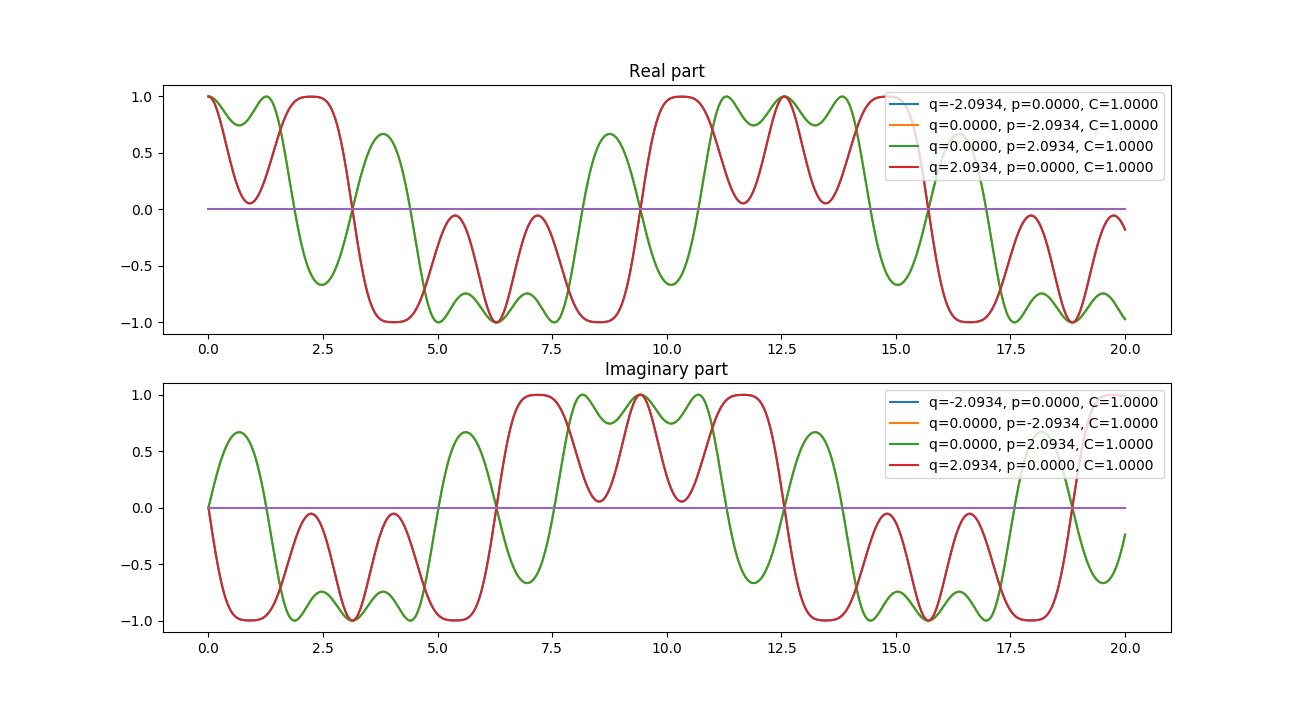
\includegraphics[scale=0.5]{eq_coeff.png}
\caption{Вид коэффициентов (уравнение \ref{eq:coeff}), описываем состояние с энергией $2.5$ с помощью подогнанного базиса, %
	 можем использовать базисные функции с параметром $\sim$ 0.25 и коэффициентами $[-1.0, 1.0, 1.0, -1.0]$. %
	 Но такой сигнатуры не получаем. }
\end{figure}

Начнем с рассмотрения базиса из одного волнового пакета.
Изучим вопрос сохранения энергии:
$$<V> = \left(\frac{m\omega}{\hbar\pi}\right)^{1/2}%
	\int \myexp{\frac{1}{\hbar}\left(-m\omega x^2 + %
					 \left(2\mathit{Re}(\xi)-%
					 \frac{\hbar}{l}\right)x + %
					 2\mathit{Re}(\eta)\right)}\,dx=$$
$$=\left(\frac{m\omega}{\hbar\pi}\right)^{1/2}%
   \int \myexp{\frac{1}{\hbar}\left(-m\omega x^2 + %
					 \left(2m\omega q-%
					 \frac{\hbar}{l}\right)x - %
					 m\omega q^2\right)}\,dx=$$
$$=\left(\frac{m\omega}{\hbar\pi}\right)^{1/2}%
   \myexp{-\frac{m\omega}{\hbar} q^2}\int\myexp{-\frac{m\omega}{\hbar}%
						\left( x^2 - 2\left(q - %
						    \frac{\hbar}{2ml\omega}%
						\right)x
						\right)}\,dx=$$
$$=\myexp{-\frac{m\omega}{\hbar}\left(q^2-%
				     \left(q-%
				     \frac{\hbar}{2ml\omega}%
				     \right)^2\right)}=$$
$$=\myexp{-\frac{q}{l}+\frac{\hbar}{4ml^2\omega}}$$
$$<T> = \frac{\hbar\omega}{2}+%
	\frac{|\xi|^2}{2m}-%
	\frac{1}{2}m\omega^2%
	\left(\frac{\hbar}{2m\omega}+%
	\left(\frac{\mathit{Re}(\xi)}{m\omega}%
	\right)^2\right)=$$
$$=\frac{\hbar\omega}{4}+%
   \frac{m^2\omega^2q^2+p^2}{2m}-%
   \frac{1}{2}m\omega^2q^2 = \frac{\hbar\omega}{4}+\frac{p^2}{2m}$$
$$<H>'_t=<V>'_t+<T>'_t=\frac{p\dot{p}}{m}-%
		       \frac{\dot{q}}{l}\myexp{-\frac{q}{l}+%
					       \frac{\hbar}{4ml^2\omega}}=$$
$$=\frac{p}{m}\left(\dot{p}-\frac{1}{l}\myexp{-\frac{q}{l}+%
					      \frac{\hbar}{4ml^2\omega}}%
	      \right)$$
Если принять, что $\dot{p} = -V'_x(q)$, то получим
$$<H>'_t=\frac{p}{lm}\myexp{-\frac{q}{l}}%
	 \left(1-\myexp{\frac{\hbar}{4ml^2\omega}}\right)$$
Если же принять, что $\dot{p}=-<V'_x>=<V>/l$, то получим $<H>'_t=0$

Базис из двух функций:
$$\mathbbm{V} = \left( \begin{matrix} %
		\myexp{-\frac{q_1}{l}+\frac{\hbar}{4ml^2\omega}} & %
		V_{12} \\ %
		V_{12}^* & %
		\myexp{-\frac{q_2}{l}+\frac{\hbar}{4ml^2\omega}} \\ %
		\end{matrix} \right)$$
$$\mathbbm{T} = \left( \begin{matrix} % 
		       \frac{\hbar\omega}{4}+\frac{p_1^2}{2m} & %
		       T_{12} \\ %
		       T_{12}^* & %
		       \frac{\hbar\omega}{4}+\frac{p_2^2}{2m} %
		       \end{matrix} \right)$$

Обобщая предыдущие рассуждения, предполагаем, 
что среднее значение энергии теперь сохраняться не будет. 
Однако, след марицы оператора Гамильтона все еще представляет собой сумму классических функций 
Гамильтона отдельных пакетов и поправки. 
Таким образом, след матрицы оператора Гамильтона будет сохраняться с течением времени.



\end{document}
